% Figure from MATH 556 notes, section 37. Compile with the notes preamble.
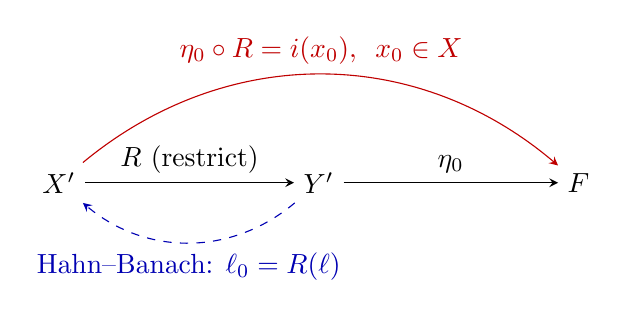
\begin{tikzpicture}[>=stealth, scale=1.1]
    \node (Xp) at (0,0) {$X'$};
    \node (Yp) at (3,0) {$Y'$};
    \node (F) at (6,0) {$\mathbb{F}$};
    \draw[->] (Xp) -- node[above] {$R$ (restrict)} (Yp);
    \draw[->] (Yp) -- node[above] {$\eta_0$} (F);
    \draw[->, red!75!black] (Xp) to[bend left=40] node[above] {$\eta_0 \circ R = i(x_0)$, \ $x_0 \in X$} (F);
    \draw[->, dashed, blue!70!black] (Yp) to[bend left=40] node[below] {Hahn--Banach: $\ell_0 = R(\ell)$} (Xp);
\end{tikzpicture}
